%----------------------------------------------------------------
%
%  File    :  survey-intro.tex
%
%  Author  :  Keith Andrews, IICM, TU Graz, Austria
% 
%  Created :  27 May 1993
% 
%  Changed :  16 Nov 2010
% 
%----------------------------------------------------------------


\chapter{Web Tools For Accessibility Audits}

\label{chap:WebTools}



Web tools for accessibility audits provide core auditing functionality
to anyone interested. The amount of tools in this category is large,
and most of these tools come to the same conclusions for an audited
web page regardless of the level of detail. This is attributed to
several factors, one being that many of these web tools are using the
same core library to assess the accessibility of a given website. In
the case of this survey, the used library is called axe-core, which is
provided by the Deque company.

In this survey, the tools that are inspected closely are but a
fraction of the tools that are currently available on the web. The
chosen tools were selected in a way, which enables a closer look at
tools that run with the axe core library and without. Additionally,
the selection also tries to show the different qualities of each
choice and what can be expected when someone tries to use these tools
online.

In this survey, our selection of web tools for accessibility audits
consists of the following: Accessi, WAVE, and Page Speed Insights
which is the web tool equivalent to the Lighthouse browser
extension. All of the mentioned web tools will be discussed in further
detail in the following sections. For each of these three tools, there
were also videos created, which demonstrates the features and the
functionality of each of the tools. The videos also give a quick
overview of the metrics that were used to determine the accessibility
of the tested websites.




\section{Accessi}

Accessi \parencite{Accessi} is one of the websites that were used to
assess the accessibility of the two test pages. Accessi is a website
that offers a free accessibility test to its users. It works according
to the Web Content Accessibility Guidelines (WCAG) standard. This can
be further refined while using the tool by a choice of the 2.0 version
of this standard or its 2018 renewed 2.1 version.  The website will
analyze the target test website and give a basic rating between
0-100\% telling the user the state of compliance of the test
site. Through an automated test, further metrics are detected, one
example being a statistical analysis of the found issues of the web
page. Accessi ranks these issues in three categories: High impact,
medium impact, and low impact. The high-impact issues are the most
obvious and intrusive ones, descending in severity, followed by medium
and low. All the issues that are detected by the automated test run
will additionally be listed, described, and enhanced with
examples. The feature that makes Accessi stand out from its
competitors is the ability to export all of the aforementioned
findings in PDF or CSV format, giving the user a form of a To-Do list
or a fixed statement that they could work on if they would be looking
towards improving the accessibility of their web site. An example of
the graphical interface of Accessi can be seen in
Figure~\ref{fig:accessi}.



\begin{figure}[tp]
\centering
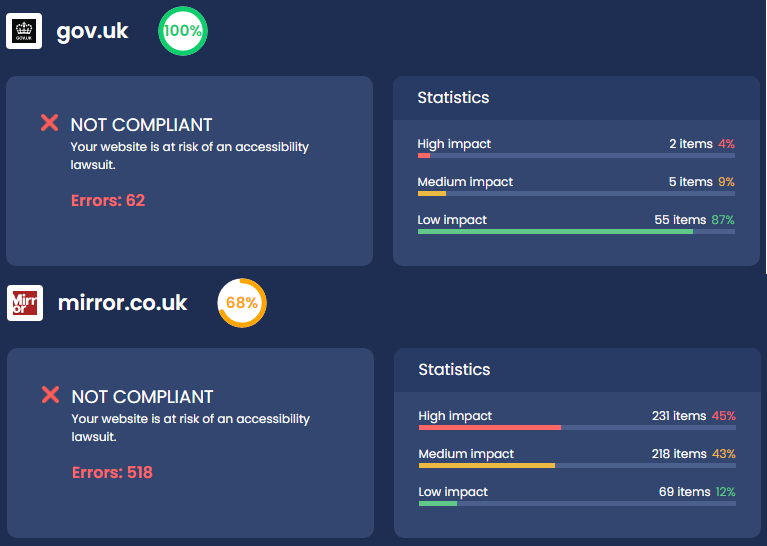
\includegraphics[keepaspectratio,width=\linewidth,height=\halfh]
{images/accessi.png}

\caption[Accessi Overview]
{%
Accessi web tool header showing an overview for each test site.
}
\label{fig:accessi}
\end{figure}





\section{WAVE}

WAVE \parencite{WAVE_web} is a tool provided by the company WebAim. As
the tools described in this survey its purpose is to assess the
accessibility of a website. WAVE offers a different take on the user
interaction with a website which is subject to an accessibility
test. The user is offered an interactive web tool, which embeds itself
in the test website which is being surveyed.  This embedded interface
gives the user the ability to interactively inspect all the errors and
warnings that are produced for a given website. The user is given the
ability to click on icons which are attatched to elements of the test
site, clearly outlining which element is considered non-compliant with
accessibility guidelines. This interactivity is a special feature of
the WAVE tool as through the course of research in our survey it is
still the only tool providing these options. The interactive nature of
the tool really provides the user with an indepth look into each error
and where on the website it is located. In addition to this feature,
WAVE also gives a summary over all the different kinds of errors or
issues find on a given website. This detailed summary is linked to the
icons that are embedded in the website that si being surveyed and will
outline and focus the element from the list on the website if clicked
on.

As can be seen in the Figure \ref{fig:WAVE} below this web tool does
not necessarily work with every website, as due to some scripting
errors the tool might fail to integrate itself properly into some
websites.


\begin{figure}[h!]
\centering
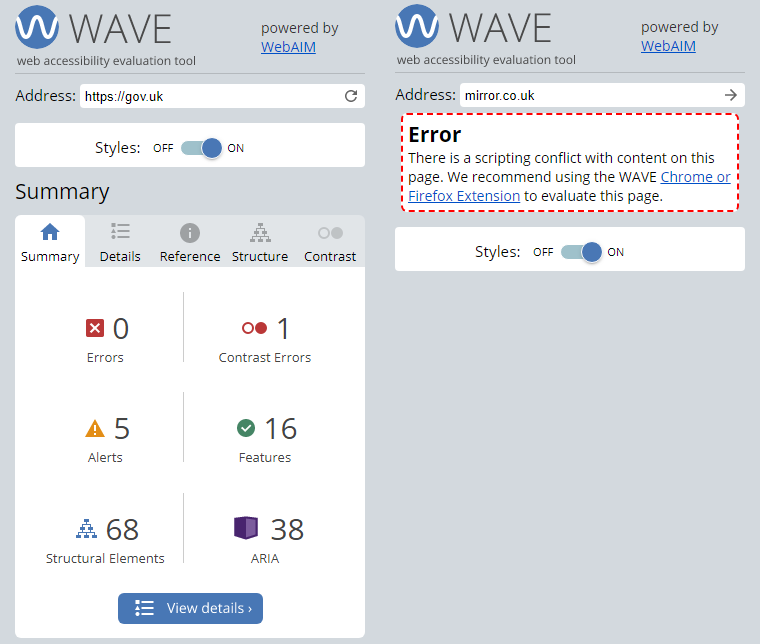
\includegraphics[keepaspectratio,width=\linewidth,height=\halfh]
{images/WAVE.png}

\caption[Accessi Overview]
{%
WAVE web tool header showing an overview for each test site.
}
\label{fig:WAVE}
\end{figure}






\section{Page Speed Insights aka. Lighthouse}

Page Speed Insights \parencite{PSIL} is a web tool based on the popular Lighthouse browser extension. Using the axe-core library as mentioned in Chapter \ref{tab:browser-extensions-info} this tool provides the same functionality as its browser extension counterpart. The tool can evaluate not only in consideration to accessibility but other metrics relevant to website quality. The web tool offers insight into basic performance, best practices, and Search Engine Optimization (SEO), in addition to assessing the accessibility of the tested website. After the accessibility audit is done the user may interact with the tool for further information on the found issues. These issues are represented in a list format, explaining what the current error is, as well as suggestions on how to fix said errors and examples of what they might look like. This list view can be seen in the given example in Figure \ref{fig:PSIL} below. Each of the elements in the list can be clicked on to view a more detailed version of the aforementioned errors and issues. 

\begin{figure}[tp]
\centering
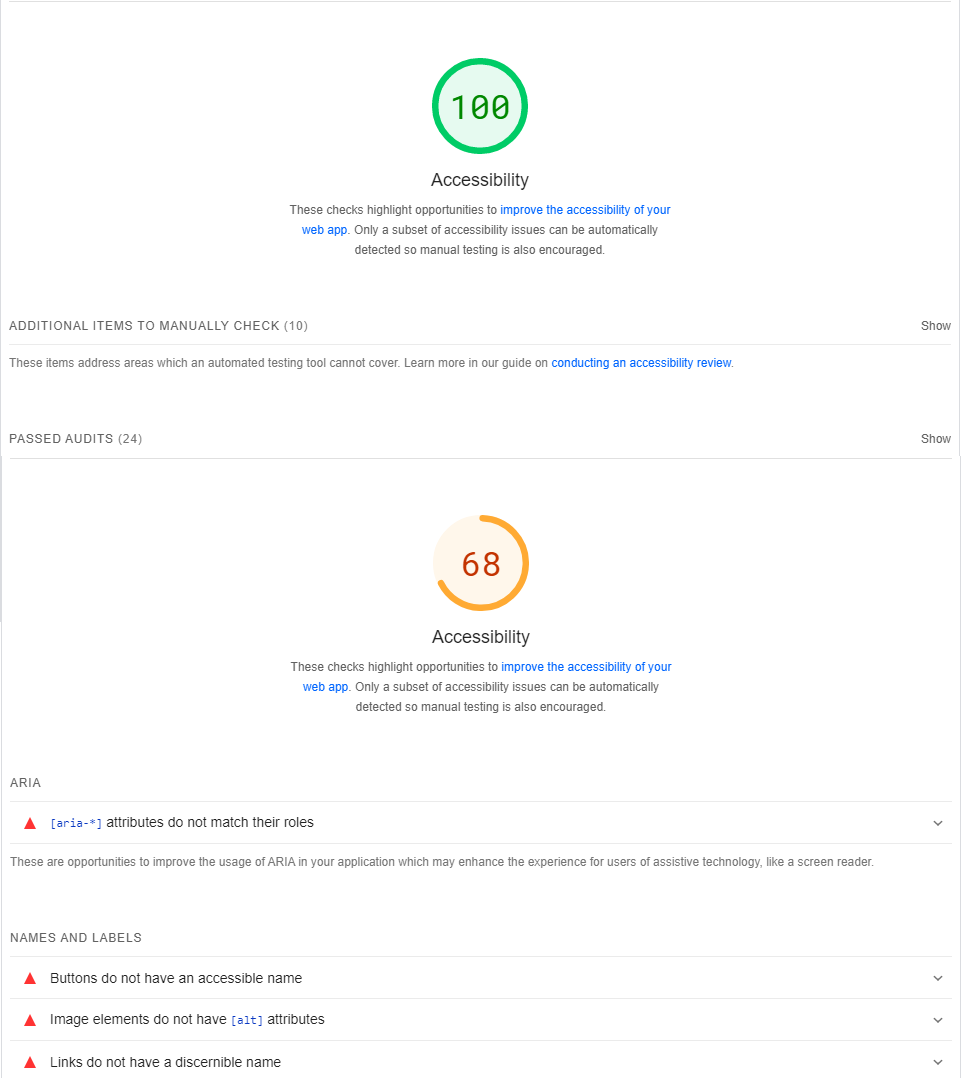
\includegraphics[keepaspectratio,width=\linewidth,height=\halfh]
{images/lighthouse.png}

\caption[Page Speed Insights Overview]
{%
Page Speed Insights (Lighthouse) web tool showing an overview for each test site.
}
\label{fig:PSIL}
\end{figure}




\section{Showcase videos}

In this survey, two websites were targeted for evaluation by the
aforementioned tools. For a good example concerning web accessibility,
the \url{https://www.gov.uk/} website was chosen whereas for the
negative example \url{https://www.mirror.co.uk/} was the choice. The
videos that were produced each showcase the interaction between the
user, the tools, and the website that is being evaluated
respectively. A video of this format was produced for Accessi
\parencite{Accessi_vid}, WAVE \parencite{WAVE_vid} and Page Speed
Insights (Lighthouse) \parencite{PageSpeedInsights_vid}. All of these
videos showcase the features of the tool that is being covered as well
as highlight a few extras the tool of each video might have over other
tools that might have a different focus. The outcome of all of the
videos is yet the same, as they all evaluate the positive example as
being very well rated and rating the negative example as being
non-compliant with the usual standards of accessibility for websites.



\section{Web Tools For Accesibility Audits Conclussion}

Concluding this chapter of the survey, its is fair to say that the
selection of web tools for accessibility audits is plentiful. There is
many tools which base themselves on the axe-core library and many
others which use their own librarys to assess the accessibility of a
website. As there is a standard in place which sets the boundarys for
accessibility usually all the tools come to the same general
conclusion for a given website, evaluating a good website as compliant
to accessibility and bad ones as being non-compliant. Through the big
selection of available tools it is adviseable to choose the one which
suits the needs of the auditor the most. An example would be when
maintaining a website on their own, the auditor might choose to use
either WAVE or Accessi, depending on if they prefer a list type of
view or the more interactive way. When looking for a more general
overview including other metrics like performance it is probably safe
to assume that Page Speed Insights will be more useful, as it always
includes a performance report as well as many other metrics
additionally to the accessibility assessment. The overall
recommendation is to first find a tool that is applicable to the
situation for each individual auditor. From this decision on the tools
commonly provide the same answer to a given test, where they focus on
different details depending on which tool was chosen.


